\section[Breve reseña histórica]{Breve reseña histórica de la utilización de las
    \gls{tic} en la educación}

El análisis de la historia de las \Gls{tic} en educación es
indispensable\cite{mcdougall2006theory}. Existe una corriente que tiende a
desestimar las experiencias pasadas, cuyo principal fundamente es la velocidad
con la que la tecnología evoluciona, es importante el estudio de la evolución de
la misma pues los errores pedagógicos cometidos, aunque puedan parecer evidentes
hoy en día, condujeron a nuevos modelos y conclusiones que son la base de la
utilización de las \Gls{tic} hoy en día\cite{mcdougall2006theory}.

La historia de las \Gls{tic} en educación comienza en la \enquote{Open
    University of United Kingdom} que en $1969$ se establece como la primera
institución educativa dedicada a la enseñanza a distancia utilizando las, para
aquel entonces, nuevas tecnologías\cite{tinio:ict}.

El impacto de las \Gls{tic} en la educación no ha sido constante durante su
historia, sino más bien, ha evolucionado de ser un medio más de traspaso de
información, hasta hoy en día, donde permite generar
conocimiento\cite{tinio:ict}.

\begin{figure}
\centering
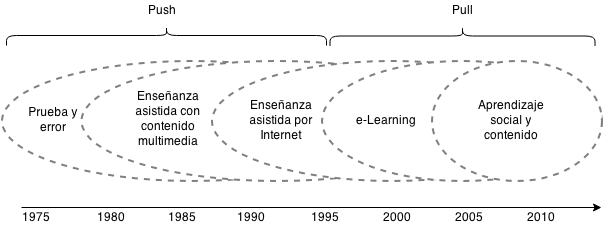
\includegraphics[scale=0.75]{tics/images/tics_history.png}
\caption{Utilización de las \Gls{tic} en la educación desde el año $1975$. Las
    fechas utilizadas son relacionadas a la evolución en los Estados Unidos de
    Norte America.}
\label{fig:history_tics}
\end{figure}

Para entender la historia de las \Gls{tic} en la educación, se presenta el
gráfico~\ref{fig:history_tics}, en el cual se observa la evolución que sufrió la
utilización de las \Gls{tic} como herramienta en la educación. Se observa que se
parte la historia en cinco corrientes definidas, y a la vez, estas corrientes se
agrupan según el mecanismo de obtención de información, las tres primeras
corrientes se denominan \textit{pull} y las siguientes dos se denominan
\textit{push}. 

El modelo de comunicación denominado \emph{Push} representa a la etapa donde los
estudiantes obtienen información sin una participación activa en la creación de
esa información\cite{white:ict}. La corrientes pedagógicas que marcan tendencia
en esta época son el instruccionismo y el
conductismo\cite{white:ict,leinonen:ict}.

La evolución de la tecnología permite mejorar los mecanismos de comunicación,
creando redes interactivas donde se comparte la información, modelo denominado
\emph{pull}. En el modelo \emph{pull} los alumnos son creadores activos de
conocimiento\cite{white:ict,leinonen:ict}, se intensifica la creación de
herramientas basadas en el constructivismo y el construccionismo. Es importante
notar que las pedagogías de la época \textit{Push}, mantienen popularidad y
siguen evolucionando\cite{white:ict}.

En el gráfico~\ref{fig:history_tics} se observa el solapamiento entre los
diversos mecanismos utilizados. Se muestra el inicio de la utilización de una
herramienta, pero no su fin, actualmente se sigue utilizando todas las
pedagogías\cite{leinonen:ict}.

Aunque la figura~\ref{fig:history_tics} muestre un progreso lineal de las
corrientes, este progreso no es igual en todo el mundo, y la el grado de impacto
de las \Gls{tic} varia entre países, lo que se conoce como una \enquote{brecha
    tecnológica}.

\observacion{Revisar estructura}
\observacion{Educación, antecedes, instruccionismo?, pero no habla de la
    evolución de instruccionismo, no da a entender en que momento pasa de una a
    otra. Colocar las corrientes en su gráfica 2.1}

